%%%%%%%%%%%%%%%%%%%%%%%%%%%%%%%%%%%%%%%%%
% Beamer Presentation
% LaTeX Template
% Version 1.0 (10/11/12)
%
% This template has been downloaded from:
% http://www.LaTeXTemplates.com
%
% License:
% CC BY-NC-SA 3.0 (http://creativecommons.org/licenses/by-nc-sa/3.0/)
%
%%%%%%%%%%%%%%%%%%%%%%%%%%%%%%%%%%%%%%%%%

%----------------------------------------------------------------------------------------
%	PACKAGES AND THEMES
%----------------------------------------------------------------------------------------

\documentclass{beamer}

\mode<presentation> {

% The Beamer class comes with a number of default slide themes
% which change the colors and layouts of slides. Below this is a list
% of all the themes, uncomment each in turn to see what they look like.

%\usetheme{default}
%\usetheme{AnnArbor}
%\usetheme{Antibes}
%\usetheme{Bergen}
%\usetheme{Berkeley}
%\usetheme{Berlin}
%\usetheme{Boadilla}
%\usetheme{CambridgeUS}
%\usetheme{Copenhagen}
%\usetheme{Darmstadt}
%\usetheme{Dresden}
%\usetheme{Frankfurt}
%\usetheme{Goettingen}
%\usetheme{Hannover}
%\usetheme{Ilmenau}
%\usetheme{JuanLesPins}
%\usetheme{Luebeck}
\usetheme{Madrid}
%\usetheme{Malmoe}
%\usetheme{Marburg}
%\usetheme{Montpellier}
%\usetheme{PaloAlto}
%\usetheme{Pittsburgh}
%\usetheme{Rochester}
%\usetheme{Singapore}
%\usetheme{Szeged}
%\usetheme{Warsaw}

% As well as themes, the Beamer class has a number of color themes
% for any slide theme. Uncomment each of these in turn to see how it
% changes the colors of your current slide theme.

%\usecolortheme{albatross}
%\usecolortheme{beaver}
%\usecolortheme{beetle}
%\usecolortheme{crane}
%\usecolortheme{dolphin}
%\usecolortheme{dove}
%\usecolortheme{fly}
%\usecolortheme{lily}
%\usecolortheme{orchid}
%\usecolortheme{rose}
%\usecolortheme{seagull}
%\usecolortheme{seahorse}
%\usecolortheme{whale}
%\usecolortheme{wolverine}

%\setbeamertemplate{footline} % To remove the footer line in all slides uncomment this line
%\setbeamertemplate{footline}[page number] % To replace the footer line in all slides with a simple slide count uncomment this line

%\setbeamertemplate{navigation symbols}{} % To remove the navigation symbols from the bottom of all slides uncomment this line
}

\usepackage{graphicx} % Allows including images
\usepackage{booktabs} % Allows the use of \toprule, \midrule and \bottomrule in tables
\usepackage{hyperref}
%----------------------------------------------------------------------------------------
%	TITLE PAGE
%----------------------------------------------------------------------------------------

\title[Paper summary]{Automatic Label-free Detection of Breast Cancer Using Nonlinear Multimodal Imaging and the Pretrained Convolutional Neural Network ResNet50 - Summary
} % The short title appears at the bottom of every slide, the full title is only on the title page

\author{Mr. Prince Adjei} % Your name
\institute[Code Lab] % Your institution as it will appear on the bottom of every slide, may be shorthand to save space
{
Connected Devices Lab \\ % Your institution for the title page
\medskip
\textit{prince.e.adjei@gmail.com} % Your email address
}
\date{\today} % Date, can be changed to a custom date

\begin{document}

\begin{frame}
\titlepage % Print the title page as the first slide
\end{frame}

\begin{frame}
\frametitle{Overview} % Table of contents slide, comment this block out to remove it
\tableofcontents % Throughout your presentation, if you choose to use \section{} and \subsection{} commands, these will automatically be printed on this slide as an overview of your presentation
\end{frame}

%----------------------------------------------------------------------------------------
%	PRESENTATION SLIDES
%----------------------------------------------------------------------------------------

%------------------------------------------------
\section{Image preprocessing} % Sections can be created in order to organize your presentation into discrete blocks, all sections and subsections are automatically printed in the table of contents as an overview of the talk
%------------------------------------------------


\begin{frame}
\frametitle{Image preprocessing and image patch extraction }
\begin{itemize}
\item  The aim of pre-processing is an improvement of the image data that suppresses unwilling distortions or enhances some image features important for further processing.
\item For the project we use several popular image preprocessing techniques.
\item The first step is to downsample the images by a factor of two. 
\item Median smoothing is performed next. (all terms will be explained next)
\item  The resulting smoothed images are then corrected for the mosaicking artifacts produced by the uneven illumination of the image tiles.
\item The last stage is to ajust image contrast via contrast limited adaptive histogram equalization algorithm (CLAHE).
\end{itemize}
\end{frame}

%------------------------------------------------
\subsection{Down sampling}
\begin{frame}
\frametitle{What at all is down sampling we talked about?}
It is essential to reduce our image sizes before feeding to the neural network. But we need an effective way to this.
\begin{block}{Down sampling}
Ever wondered how to resize an image? Simple – throw away data. When “shrinking” an image’s dimensions (note: this is NOT the same as image compression), you are essentially throwing away image information.
\end{block}

\begin{itemize}
    \item Suppose you have an image with dimensions AxB, and you want to shrink it to the dimensions of CxD, assuming that A$>$C and B$>$D.
    \item The most straightforward way to do this is to discard entire columns$/$rows of data. How do we know which ones to discard though?
    
\end{itemize}
\end{frame}

%------------------------------------------------
%------------------------------------------------

\begin{frame}
\frametitle{More on Down Sampling}
\begin{itemize}
   \item For the sample image shown below, we delete the first (A-C) columns, and the first (B-D) rows. The result is less than desirable.
   \item We have  effectively cropped out a large portion of the original image.
\end{itemize}
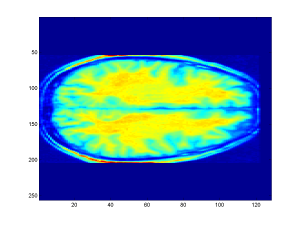
\includegraphics[scale=0.5
]{standard.png}
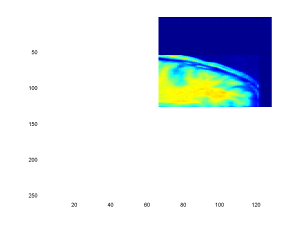
\includegraphics[scale=0.5
]{cropped.png}
\end{frame}

%------------------------------------------------
%------------------------------------------------

\begin{frame}
\frametitle{More on Down Sampling}
\begin{itemize}
   \item So, what approach should we take? Simple! First, calculate the number of columns you will need to discard, k. 
   \item Since the original number of columns is A, and the new number of columns is C, it only makes sense that we need to discard (A-C) columns.
   \item The columns and rows marked for deletion are represented with white lines, as shown below
   \item Once we’ve processed/generated the final output image, we get the following:
\end{itemize}
\end{frame}

%------------------------------------------------
%------------------------------------------------

\begin{frame}
\frametitle{More on Down Sampling}
\begin{itemize}
   \item Just to drive the point home, I must again emphasize that image data has been permanently lost, but however we have a preferable situation compared to the first case where we just cut some part of the image. 
\end{itemize}
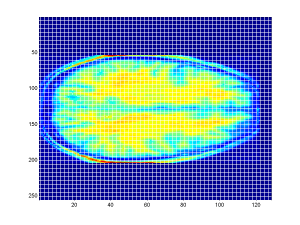
\includegraphics[scale=0.5
]{fordeletion.png}
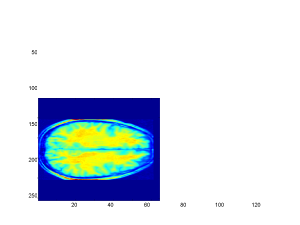
\includegraphics[scale=0.5
]{downsampled.png}
\end{frame}

%------------------------------------------------
%------------------------------------------------
\subsection{Median smoothing}
\begin{frame}
\frametitle{Median Smoothing}
\begin{itemize}
   \item So, we have effectively discussed down sampling. Now let us focus on the second stage of in our preprocessing pipeline (median smoothing).
   \item The Median Filter is a non-linear digital filtering technique, often used to remove noise from an image or signal.
   \item Such noise reduction is a typical pre-processing step to improve the results of later processing (for example, edge detection on an image). 
   \item Median filtering is very widely used in digital image processing because, under certain conditions, it preserves edges while removing noise.
   \item The main idea of the median filter is to run through the signal entry by entry, replacing each entry with the median of neighboring entries.
\end{itemize}
\end{frame}

%------------------------------------------------
%------------------------------------------------

\begin{frame}
\frametitle{Median Smoothing}
\begin{itemize}
   \item The pattern of neighbors is called the "window", which slides, entry by entry, over the entire signal.
   \item  For 1D signals, the most obvious window is just the first few preceding and following entries. 
   \item For 2D (or higher-dimensional) data the window must include all entries within a given radius or ellipsoidal region
\end{itemize}
\begin{figure}
    \centering
    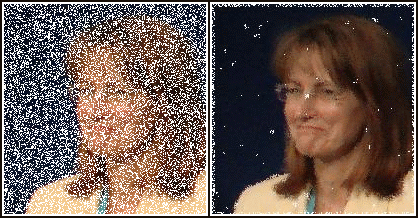
\includegraphics[scale=0.45]{medianfilter.png}
    \caption{Use of a median filter to improve an image severely corrupted by defective pixels}
    \label{fig:median_filter}
\end{figure}
\end{frame}

%------------------------------------------------
%------------------------------------------------
\subsection{Contrast adjustment}
\begin{frame}
\frametitle{Adjusting For Contrast}
\begin{itemize}
   \item After correcting for uneven illumination the nest step is to adjust the image contrast.
   \item  We do this via contrast limited adaptive histogram equalization algorithm (CLAHE). 
   \item Adaptive  Histogram Equalization (AHE) is a computer image processing technique used to improve contrast in images. 
   \item It differs from ordinary histogram equalization in the respect that the adaptive method computes several histograms, each corresponding to a distinct section of the image, and uses them to redistribute the lightness values of the image. 
   \item It is therefore suitable for improving the local contrast and enhancing the definitions of edges in each region of an image.
\end{itemize}
\end{frame}

%------------------------------------------------
%------------------------------------------------

\begin{frame}
\frametitle{Contrast Limited AHE}
\begin{itemize}
   \item Ordinary AHE tends to overamplify the contrast in near-constant regions of the image, since the histogram in such regions is highly concentrated.
   \item  As a result, AHE may cause noise to be amplified in near-constant regions. 
   \item  Contrast Limited AHE (CLAHE) is a variant of adaptive histogram equalization in which the contrast amplification is limited, so as to reduce this problem of noise amplification.
\end{itemize}
\begin{figure}
    \centering
    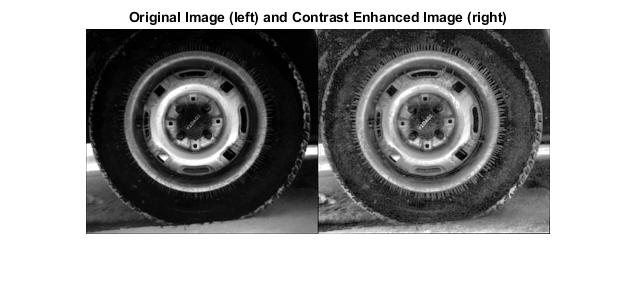
\includegraphics[scale=0.4]{clahe.png}
\end{figure}
\end{frame}

%------------------------------------------------
%------------------------------------------------
\subsection{Patch extraction}
\begin{frame}
\frametitle{Patch Extraction}
\begin{itemize}
   \item After the images preprocessing, the obtained multimodal image was compared with the corresponding annotated H \& E image that describe three different regions within the patient tissues.
   \item These regions denote to the cancerous, fat, and normal breast tissue.
   \item   Thereafter, each multimodal image was sliced into patches of the size 512 $\times$ 512 pixels.
   \item Only the patches that have a specific one tissue label were selected for the further analysis.
\end{itemize}

\end{frame}

%------------------------------------------------
%------------------------------------------------

\section{Patch Classification}
\begin{frame}
\frametitle{Patch Classification}
\begin{itemize}
   \item The selected patches from the multimodal image were utilized to check the quality of two machine learning (ML) algorithms in detecting the breast cancerous tissues. 
   \item These algorithms represent examples of the main two approaches in ML: The classical machine learning approach and the deep learning approach. 
   \item  For the classical machine learning, the patch classification was accomplished using a linear discriminant analysis (LDA) model.
   \item The deep convolutional neural network ResNet50 was utilized as a representative of the deep learning approach
\end{itemize}

\end{frame}

%------------------------------------------------
%------------------------------------------------

\subsection{Neural Networks}
\begin{frame}
\frametitle{What are Neural Networks?}
\begin{itemize}
   \item A neural network is exactly what it says in the name. It is a network of neurons that are used to process information. 
   \item To create these, scientists looked at the most advanced data processing machine at the time — the brain.
   \item Our brains process information using networks of neurons.
   \item   They receive an input, process it, and accordingly output electric signals to the neurons it is connected to. \item Using bio-mimicry, we were able to apply the architecture of our brains to further the field of artificial intelligence.
   
\end{itemize}
\centering
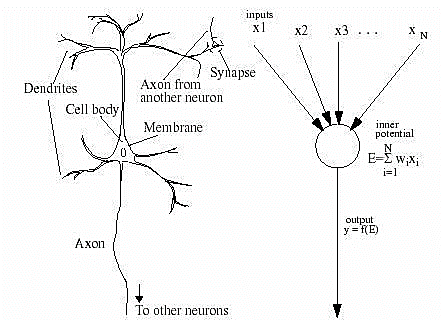
\includegraphics[scale=0.3]{ann.png}
\end{frame}

%------------------------------------------------
%------------------------------------------------


\begin{frame}
\frametitle{The parts of a neural network}
\centering
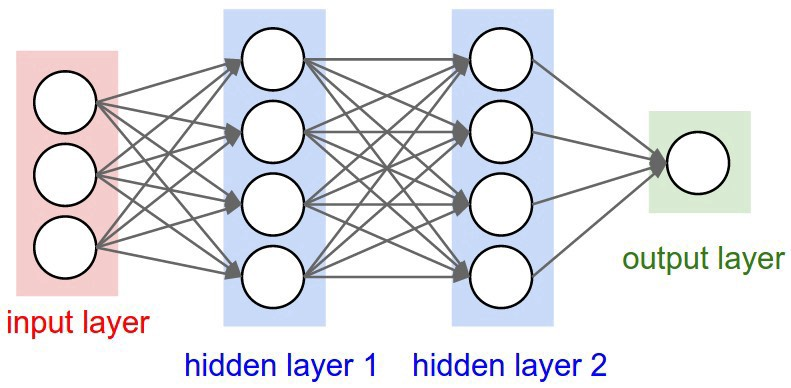
\includegraphics[scale=0.2]{partsnn.jpeg}
\begin{itemize}
   \item A neural network is made up of 3 main parts.
   \item \textbf{Input layer} - 
This is literally the layer that inputs information for the neural network to process. Each circle represents 1 feature (a piece of information). 
  
  
   
\end{itemize}

\end{frame}

%------------------------------------------------
%------------------------------------------------


\begin{frame}
\frametitle{The parts of a neural network}
\centering
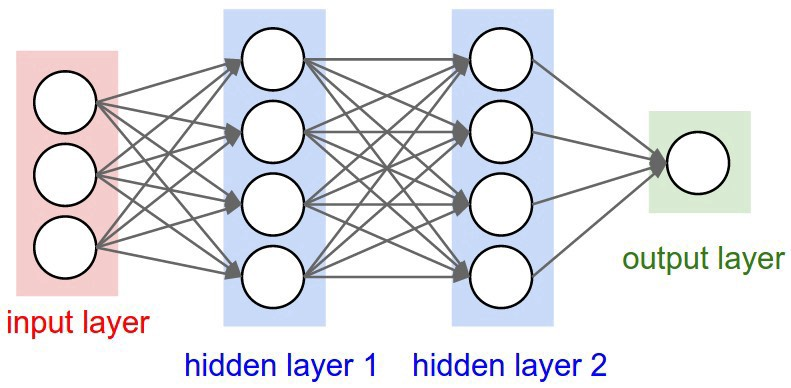
\includegraphics[scale=0.2]{partsnn.jpeg}
\begin{itemize}
   
   \item \textbf{Hidden layers} - These layers do all the processing for neural networks. 
   
   \item You can have as many of these as you want. 
   
   \item Generally speaking, the more hidden layers you have, the more accurate the neural network will be. 
   
   \item Each layer consists of nodes that mimic our brains’ neurons.
   
   \item These nodes receive information from the previous layer’s nodes, multiply it by weight and then add a bias to it. Each line in the diagram represents a weight. 
  
   
\end{itemize}

\end{frame}

%------------------------------------------------
%------------------------------------------------


\begin{frame}
\frametitle{The parts of a neural network}
\centering
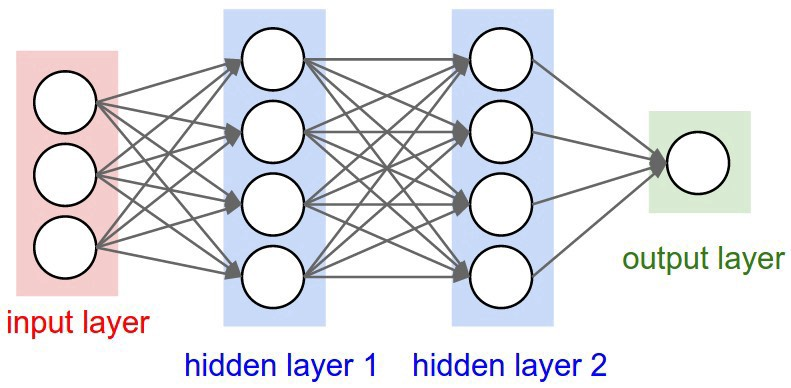
\includegraphics[scale=0.2]{partsnn.jpeg}
\begin{itemize}
   
   \item \textbf{Output layers} -This layer simply brings together the information from the last hidden layer of the network to output all the information you need from the program.
   
  
   
\end{itemize}

\end{frame}

%------------------------------------------------
%------------------------------------------------

\subsection{Convolutional Neural Networks}
\begin{frame}
\frametitle{Understanding CNNs}

\begin{itemize}
   
   \item In neural networks, Convolutional neural network (ConvNets or CNNs) are one of the main categories to do image recognition, image classifications. 
   \item Inorder to keep the presentation a little shorter I have attached a very helpful link on CNNs and will focus on explaining resnet-50
   
   \item \url{https://towardsdatascience.com/simple-introduction-to-convolutional-neural-networks-cdf8d3077bac}
   
  
   
\end{itemize}

\end{frame}

%------------------------------------------------
%------------------------------------------------

\subsection{Resnet}
\begin{frame}
\frametitle{Intuition behind Residual Networks}

\begin{itemize}
   
   \item There are a couple of intuitions that we should understand before getting into the mechanics of ResNets. 
   \item Given a shallower network - how can we take it, add extra layers and make it deeper - without losing accuracy or increasing error? 
   \item It’s tricky to do but one insight is that if the extra layers added to the deeper network are identity mappings, they become equivalent to the shallower network.
   \item And hence, they should produce no higher training error than it’s shallower counterpart.
   \item This is called a solution by construction by the authors.
\end{itemize}

\end{frame}

%------------------------------------------------
%------------------------------------------------

\begin{frame}
\frametitle{Understanding Residual}

\begin{itemize}
   
   \item A residual is the error in a result. 
  
\end{itemize}
\begin{example}[Illustration]
Let’s say, you are asked to predict the age of a person, just by looking at her. If her actual age is 20, and you predict 18, you are off by 2. 2 is our residual here. If you had predicted 21, you would have been off by -1, our residual in this case. In essence, residual is what you should have added to your prediction to match the actual.
\end{example}
\begin{itemize}
    \item What is important to understand here is that, if the residual is 0, we are not supposed to do anything to the prediction. We are to remain silent since the prediction already matched the actual.
\end{itemize}
\end{frame}

%------------------------------------------------
%------------------------------------------------

\begin{frame}
\frametitle{Understanding Residual}

\begin{itemize}
   
   \item This can be put into a nice little diagram.
  
  
\end{itemize}
\centering
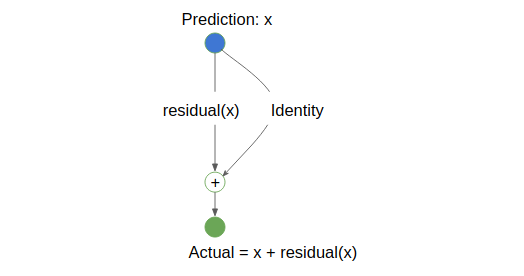
\includegraphics[scale=0.5]{resnet.PNG}

\begin{itemize}
    \item In the diagram, x is our prediction and we want it to be equal to the Actual. 
    \item However, if is it off by a margin, our residual function residual() will kick in and produce the residual of the operation so as to correct our prediction to match the actual.
    \item If x == Actual, residual(x) will be 0. The Identity function just copies x.
\end{itemize}
\end{frame}

%------------------------------------------------
%------------------------------------------------

\begin{frame}
\frametitle{The Residual Network}

\begin{itemize}
   
   \item We can now weave the above two intuitions together to come to the logical conclusion of a ResNet.
   \item We want to go deeper without degradation in accuracy and error rate. We can do this via injecting identity mappings.
    \item We want to be able to learn the residuals so that our predictions are close to the actuals.
    \item That’s what the Residual Network does. This is realized by feedforward neural network with shortcut connections.
  
  
\end{itemize}
\begin{figure}
    \centering
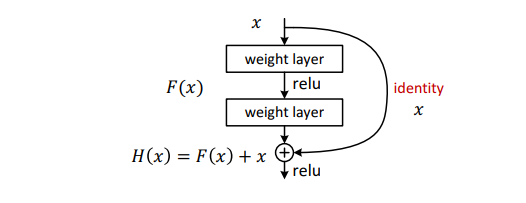
\includegraphics[scale=0.5]{resnet1.PNG}
    \caption{The reusable residual network}
    \label{fig:my_label}
\end{figure}

\end{frame}

%------------------------------------------------
%------------------------------------------------

\begin{frame}
\frametitle{The Residual Network}

\begin{itemize}
   
   \item The network can be mathematically depicted as:

$$H(x) = F(x) + x, where F(x) = W2*relu(W1*x+b1)+b2$$
\item During training period, the residual network learns the weights of its layers such that if the identity mapping were optimal, all the weights get set to 0.
\item In effect F(x) become 0, as in x gets directly mapped to H(x) and no corrections need to be made.
\item Hence these become your identity mappings which help grow the network deep.
\item if there is a deviation from optimal identity mapping, weights and biases of F(x) are learned to adjust for it. \item Think of F(x) as learning how to adjust our predictions to match the actuals.
  
  
\end{itemize}


\end{frame}


\section{Results}
%------------------------------------------------

\begin{frame}
\frametitle{Results}
\begin{itemize}
   \item LOPO-CV, patches of one patient is used as the test set and the classifier is trained and validated using the patches of the remaining patients. This is repeated for all patient image patches.
   \item For the training-test validation method, the dataset is divided into training, validation and test set which are independent of each other.
   \item The training set is used to train the classifier, the hyperparameters of the model are optimised using the validation test and the model is evaluated on the test set.
\end{itemize}
\end{frame}

%------------------------------------------------
\section{Results}
%------------------------------------------------

\begin{frame}
\frametitle{Results}
\begin{itemize}
   \item Principal component analysis is one of the statistical techniques used. It is a technique that is used to analyze the interrelationships among a large number of variables and to explain these variables in terms of a smaller number of variables, called principal components, with a minimum loss of information.
   \item In the first validation method, Principal Component Analysis(PCA) and Linear Discriminant Analysis(LDA) methods are applied(PCA-LDA) to reduce the dimensions of the features extracted by the ResNet50 model.
   \item In the second validation method, only the ResNet50 model was used and hyper parameters fine tuned on the test data.
\end{itemize}
\end{frame}

%------------------------------------------------

\begin{frame}
\frametitle{Results}
\begin{itemize}
   \item For the training-test validation method, the dataset is divided into training, validation and test set which are independent of each other.
   \item The training set is used to train the classifier, the hyperparameters of the model are optimised using the validation test and the model is evaluated on the test set.
   \item For both validation methods, this ResNet50 network was trained for 20 epochs using the Adam optimizer with a learning rate of 0.001 and categorical cross entropy as loss function.  
\end{itemize}
\end{frame}

%------------------------------------------------


\end{document} 